\documentclass[12pt]{article}
\usepackage[english]{babel}
\usepackage[utf8x]{inputenc}
\usepackage{amsmath}
\usepackage{graphicx}
\usepackage[colorinlistoftodos]{todonotes}
\usepackage{placeins}
\usepackage{makeidx}
\usepackage[export]{adjustbox}
\usepackage{caption}
\usepackage{subcaption}

\makeindex


\begin{document}

\begin{titlepage}

\newcommand{\HRule}{\rule{\linewidth}{0.5mm}} % Defines a new command for the horizontal lines, change thickness here

\center % Center everything on the page
 
%----------------------------------------------------------------------------------------
%	HEADING SECTIONS
%----------------------------------------------------------------------------------------

\textsc{\LARGE Universidade de Évora}\\[1.5cm] % Name of your university/college
\textsc{\Large Disciplina de Teoria de Informação}\\[0.5cm] % Major heading such as course name
%\textsc{\large Minor Heading}\\[0.5cm] % Minor heading such as course title

%----------------------------------------------------------------------------------------
%	TITLE SECTION
%----------------------------------------------------------------------------------------

\HRule \\[0.4cm]
{ \huge \bfseries Sistema de Compressão e Descompressão de Imagens}\\[0.4cm]
\HRule \\[1.5cm]
 
%----------------------------------------------------------------------------------------
%	AUTHOR SECTION
%----------------------------------------------------------------------------------------


\includegraphics[scale=1.1]{logo.png}\\[2cm]

\begin{minipage}{0.4\textwidth}
\begin{flushleft} \large
\emph{Autores:}\\
José Ferreira nº 34145\\
Daniel Soares nº 34222
\end{flushleft}
\end{minipage}\\[0.5cm]

\begin{minipage}{0.4\textwidth}
\begin{flushleft} \large
\emph{Docente:} \\
Miguel Barão
\end{flushleft}
\end{minipage}\\[2cm]

{\large \today}\\[2cm]

\vfill
\end{titlepage}


\thispagestyle{empty}
\renewcommand\contentsname{Índice}
\tableofcontents
\newpage
\index{Introdução}


\printindex
\section{Introdução}
No contexto da disciplina de Teoria de Informação é pretendido que com o uso de um algoritmo de compressão, seja possível comprimir e descomprimir uma imagem guardada com formato PBM (Portable BitMap). Para além destas funções existe a necesidade de determinar a sua entropia, entropia condicional e o desempenho do sistema de compressão escolhido. Sobre estes dados será necessário realizar uma analíse e retirar as devidas conclusões. Para tal objectivo foi escolhido o algoritmo de compressão LZW (Lempel-Ziv-Welch). O LZW é um algoritmo de compressão que deriva do algoritmo LZ78, baseado na localização e no registo das padronagens de uma estrutura. Este algoritmo é geralmente usado em imagens em que não se pode perder a definição original. 

\newpage
\index{Compressão}

\printindex
\section{Compressão}
Tal como referido anteriormente o algoritmo de compressão utilizado foi o LZW. Este utiliza repetição de padrões de forma a poupar espaço.
São inseridos numa fase inicial os símbolos iniciais como as primeiras duas entradas do dicionário. 
O algoritmo vai então tentar extender o dicionário criado inicialmente com novos e únicos símbolos, há medida que estes vão aparecendo na informação a comprimir, criados com combinações de símbolos já existentes no dicionário. Este método pode ser utilizado tanto para compressões como para descompressões.\\[0.5cm]
Escolheu-se este algoritmo de compressão pois para além de ser competente para imagens possui uma implementação simples e de fácil compreensão. \\[0.5cm]

\begin{center}
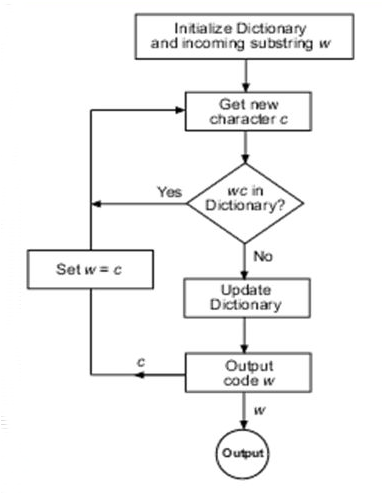
\includegraphics[scale=0.7]{compressor.png}\\[2cm]
\end{center}

\newpage
\index{Descompressão}

\printindex
\section{Descompressão}
O algoritmo escolhido também é resposavel pelo o trabalho de descompressão. O dicionário na fase inicial, do processo de descompressão, encontra-se cheio com todos os símbolos do alfabeto (0 e 1). Ele vai descodificando o ficheiro recebido, lendo o actual (a) e o proximo (p). Se p se encontrar no dicionario, é criada uma nova entrada composta por a + o primeiro símbolo de p, e esta é inserida na última posição do dicionário. Se p corresponde a uma entrada não existente no dicionario, cria-se uma entrada composta com o primeiro simbolo de a + a, e esta é inserida na última posição do dicionário. Desta forma o ficheiro vai sendo descomprimido acompanhando o crescimento do dicionário até que este possua todos os símbolos(combinações dos símbolos iniciais) do ficheiro.\\[0.5cm]

\begin{center}
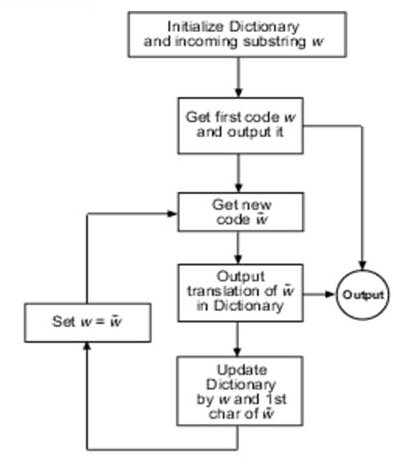
\includegraphics[scale=0.7]{descompressor.png}\\[2cm]
\end{center}	

\newpage
\index{Cálculos}

\printindex
\section{Cálculos}
\printindex
\subsubsection{Performance}
A performance é obtida fazendo a diferena entre o tamanho do array original e o número de digitos do ficheiro comprimido e em seguida é feita uma divisão pelo tamanho do array original e uma multiplicação por 100. Isto permite saber qual a percentagem do ficheiro que foi comprimida.

\begin{center}
\[ p = \frac{t_{a}-n_{d}}{t_{a}}\ \ \textrm{* 100}  \]
\end{center}

\printindex
\subsubsection{Entropia}
A entropia é uma medida de incerteza, ou seja trata-se da medida da surpresa gerada por uma fonte. Neste caso permite saber a surpresa gerada por os bits da imagem.


\begin{center}
\[ H = \Sigma\  \textrm{p(x) * log(p(x))}  \]
\end{center}


\printindex
\subsubsection{Entropia Condicional}
A entropia condicional permite medir a incerteza de uma variavel sabendo a ocorrência anterior.

\begin{center}
\[ H_{condicional} = \Sigma\textrm{p(x)} \Sigma\textrm{p(yIx) * log(p(yIx))}  \]
\end{center}

\newpage
\index{Conclusão}

\printindex
\section{Conclusão}
Depois de analisados os resultados obtidos atravez da performance, entropia e entropia condicional foi possivel chegar ás seguintes conclusões:

\subsubsection{Performance}
Neste caso podemos verificar que ela será tanto maior quanto mais repetições de pixeis sequênciais que ocorrerem e outro factor influente será as dimensões das imagens. Ou seja, frequentemente quanto maior a imagem original maior será a performance do programa.

\begin{figure}[htb!]
    \centering
    \begin{minipage}{0.45\textwidth}
        \centering
        
\includegraphics[width=0.9\textwidth]{red.png}
        \caption{Imagem maior}
    \end{minipage}\hfill
    \begin{minipage}{0.45\textwidth}
        \centering
        
\includegraphics[width=0.9\textwidth]{redpequeno.png} 
        \caption{Imagem pequena}
    \end{minipage}
\end{figure}
\centering
Fig.2 trata-se de um corte de Fig.1. Fig.1 tem p = 99.4\% e Fig.2 tem p = 98.5\%.
\flushleft
\newpage
\subsubsection{Entropia}
Depois de testar diversos casos chegou-se á conclusão que a entropia varia com a informação contida nas imagens. Imagens com vários detalhes possuem niveís de entropia maiores e imagens mais simples entropias menores. Por isso conclui-se que entropias maiores correspondem a imagens com mais elementos presentes(com maior nível de detalhe).

\begin{figure}[htb!]
    \centering
    \begin{minipage}{0.45\textwidth}
        \centering
        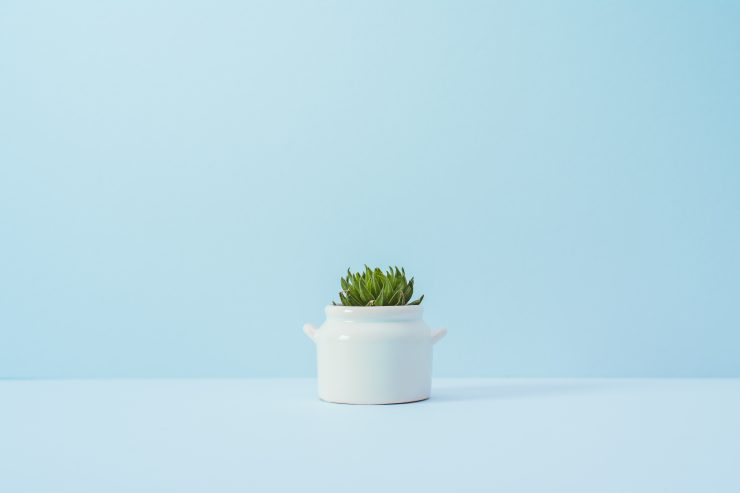
\includegraphics[width=0.9\textwidth]{simples.jpg}
        \caption{Imagem mais simples}
    \end{minipage}\hfill
    \begin{minipage}{0.45\textwidth}
        \centering
        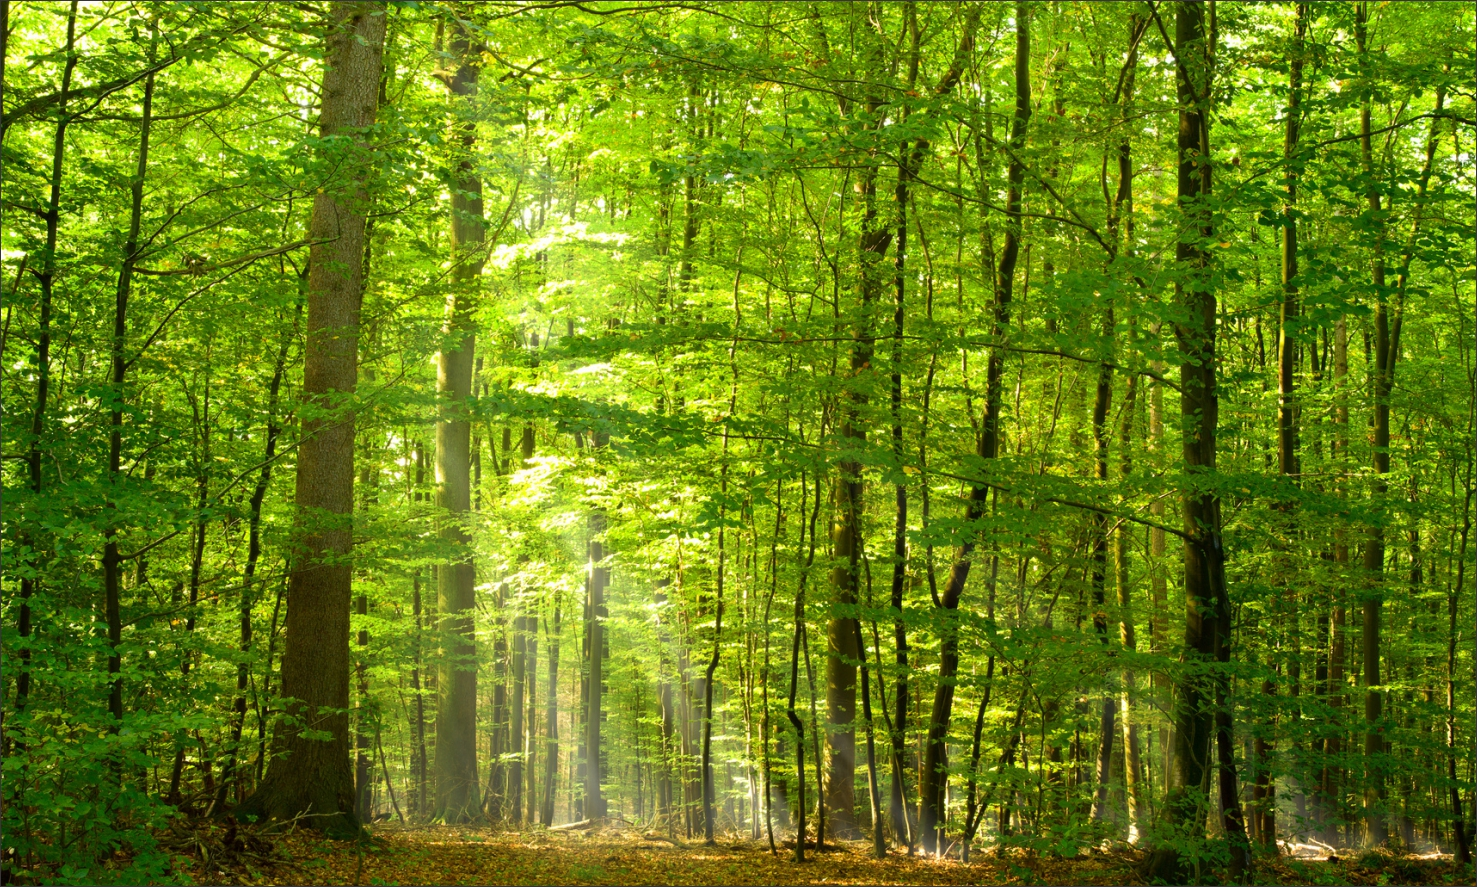
\includegraphics[width=0.9\textwidth]{floresta.jpg} 
        \caption{Imagem mais complexa}
    \end{minipage}
\end{figure}
\centering
Neste caso a Fig.3 possui H=0.20 e a Fig.4 possui H=0.95.
\flushleft
\newpage
\subsubsection{Entropia Condicional}
Ao calcular a entropia condicional estaremos a assumir que se conhece um evento logo a entropia condicional vai ser a medida de nova informação adequirida depois de um evento ser observado. Esta é menor que a entropia, devido há existência de menos incerteza pois já se conhece o bit anterior. Depois da observação de vários exemplos chegou-se á conclusão que mesmo para imagens com entropias muito semelhantes, ocorria uma maior variação entre a entropia e a entropia condicional na presença de padrões bem definidos. Quanto mais bem definido é o padrão menor é a sua entropia condicional.

\begin{figure}[htb!]
    \centering
    \begin{minipage}{0.45\textwidth}
        \centering
        
\includegraphics[width=0.9\textwidth]{padrao2.jpg}
        \caption{Imagem com padrão bem definido}
    \end{minipage}\hfill
    \begin{minipage}{0.45\textwidth}
        \centering
        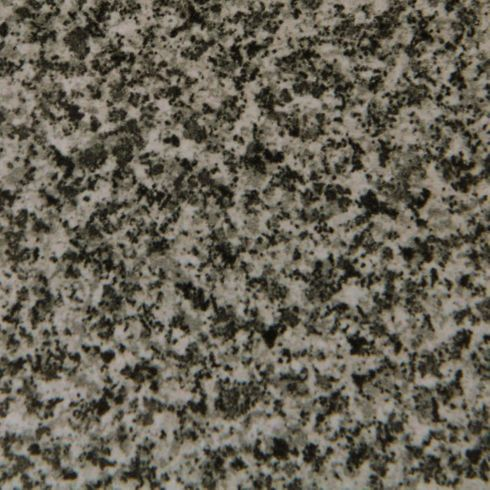
\includegraphics[width=0.9\textwidth]{granito.jpg} 
        \caption{Imagem sem nenhum padrão}
    \end{minipage}
\end{figure}

\centering
Neste caso a Fig.5 possui H=0.98 e uma H\_condicional=0.55 e a Fig.6 possui H=0.99 e uma H\_condicional=0.82.

\end{document}